\begin{figure*}
\vspace{-5mm}
\centering
\captionsetup[subfigure]{margin={-20mm,-5mm}}
\begin{subfigure}[b]{0.48\textwidth}
    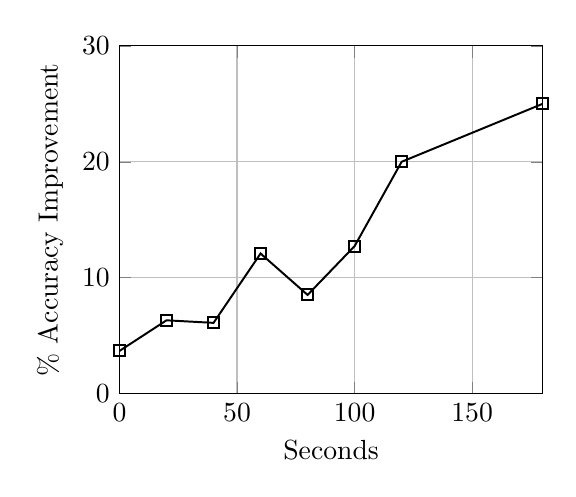
\begin{tikzpicture}
    \begin{axis}[
        % width=12cm, 
        height=6cm,
        xlabel={Seconds},
        ylabel={\% Accuracy Improvement},
        %title={(a) LLaVA Backbone on NeXT-QA},
        xmin=0, xmax=180,
        ymin=0, ymax=30,
        % xtick={5000, 10000, 15000, 20000,25000,30000, 35000},
        % xticklabels={5K, 10K, 15K, 20K, 25K,30K, 35K},
        %ytick={60, 62, 64, 66, 68, 70, 72, 74},
        legend pos=south west,
        grid=both,
        scaled ticks = false,
        scaled x ticks = false,
    ]
\addplot[line width=.25mm, color=black, mark=square, mark size=2pt]
coordinates {
(0, 3.69)
(20, 6.33)
(40, 6.11)
(60, 12.09)
(80, 8.52)
(100, 12.73)
(120, 20)
(180, 25)
};
    \end{axis}
    \end{tikzpicture}
    \caption{LLaVA Backbone on NeXT-QA.}
% \caption{Figure 1}
\end{subfigure}
\hfill
\begin{subfigure}[b]{0.48\textwidth}
    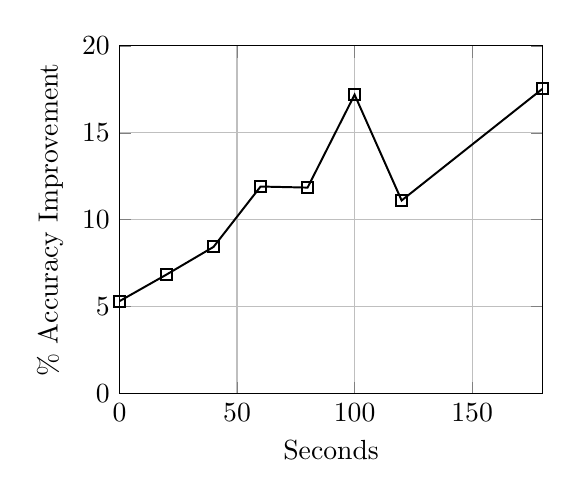
\begin{tikzpicture}
    \begin{axis}[
        % width=12cm, 
        height=6cm,
        xlabel={Seconds},
        ylabel={\% Accuracy Improvement},
        %title={(b) LLaMA Backbone on NeXT-QA},
        xmin=0, xmax=180,
        ymin=0, ymax=20,
        % xtick={5000, 10000, 15000, 20000,25000,30000, 35000},
        % xticklabels={5K, 10K, 15K, 20K, 25K,30K, 35K},
        % ytick={60, 62, 64, 66, 68, 70, 72, 74},
        legend pos=south west,
        grid=both,
        scaled ticks = false,
        scaled x ticks = false,
    ]
    % BIMBA Data

\addplot[line width=.25mm, color=black, mark=square, mark size=2pt]
coordinates {
(0, 5.32)
(20, 6.85)
(40, 8.44)
(60, 11.91)
(80, 11.85)
(100, 17.19)
(120, 11.11)
(180, 17.54)
};
    \end{axis}
    \end{tikzpicture}
    \caption{LLaMA Backbone on NeXT-QA.}
\end{subfigure}
\vspace{-3mm}
\caption{Relative performance improvement of (left) \modelLlava\ over PLLaVA baseline and (right) \modelLlama\ over LLaMA-3.2 (video) baseline for different video durations on NextQA dataset. Our model achieves larger gains as the video length increases.}
\label{fig:performance duration nextqa}
\end{figure*}



